\section{Grundlagen}
Für das Verständnis der im Projekt eingesetzten Technologien und deren Zusammenspiel ist es notwendig, zunächst die zugrunde liegenden technischen Komponenten und Frameworks näher zu erläutern. 
Dieses Kapitel stellt die wesentlichen Grundlagen vor, die für die Entwicklung des Systems relevant sind. 
Dazu zählen sowohl die verwendete Hardwareplattform in Form des TurtleBot3 als auch das Software-Framework ROS 2, das als zentrale Entwicklungsumgebung dient. 
\subsection{Turtlebot3}
Der TurtleBot3 ist ein kompakter, kostengünstiger und modular erweiterbarer mobiler Roboter, der auf dem Robot Operating System (ROS) basiert. 
Er wurde für Anwendungen in den Bereichen Forschung, Lehre, Prototypenentwicklung sowie für den hobbymäßigen Robotik-Einsatz konzipiert. 
Ziel des Turtlebot3 ist es, eine robuste, funktionsreiche und zugleich leicht zugängliche Lösung bereitzustellen, die sowohl in akademischen als auch industriellen Kontexten einsetzbar ist.
\cite{tb3_overview}\cite{tb3_home}
\newPar
Der Aufbau des TurtleBot3 ist in \imageref{tb3_components} veranschaulicht.
Als zentrale Recheneinheit verwendet der TurtleBot3 einen Raspberry Pi 4, einen leistungsfähigen und weit verbreiteten Einplatinencomputer (SBC).
Zur Umgebungswahrnehmung ist der Roboter mit einem 360°-LiDAR-Sensor ausgestattet, der präzise Abstandsmessungen und Kartierung ermöglicht. 
Darüber hinaus sind verschiedene optionale Sensoren wie Ultraschall- oder Infrarotsensoren integrierbar. 
Die mechanische Plattform ist modular aufgebaut und besteht aus leichtgewichtigen, teilweise 3D-gedruckten Komponenten, die eine einfache Anpassung und Erweiterung ermöglichen.
Das in dieser Arbeit verwendete TurtleBot3 Burger-Modell hat eine Größe von etwa \SI{14}{\centi\meter}~$\times$~\SI{18}{\centi\meter}~$\times$~\SI{19}{\centi\meter} und zeichnet sich zusätzlich durch eine maximale Geschwindigkeit von \SI{0,22}{\meter\per\second} aus.
\cite{tb3_specifications}\cite{tb3_overview}
\newPar
\begin{figure}[H]
    \centering
    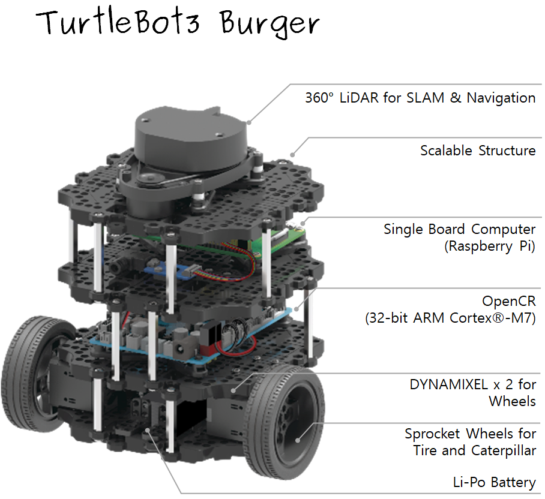
\includegraphics[width=10cm]{turtlebot3_burger_components}
    \caption{Turtlebot3 Burger Komponenten \cite{tb3_specifications}}\label{tb3_components}
\end{figure}
Technologisch unterstützt der TurtleBot3 zentrale Funktionen wie Simultaneous Localization and Mapping (SLAM) und autonome Navigation, wodurch der Roboter in der Lage ist, Umgebungen selbstständig zu kartieren und sich sicher darin zu bewegen. 
Die Steuerung kann über diverse Schnittstellen erfolgen, beispielsweise durch einen Laptop, ein Gamepad oder Android-basierte Endgeräte, was eine flexible Bedienung ermöglicht.
Zur mobilen und kabellosen Nutzung erfolgt die Energieversorgung über einen LiPo-Akku mit 1.800 mAh.
\cite{tb3_home}\cite{tb3_specifications}
\newPar
Da der Turtlebot3 von sich aus nicht über eine Kamera verfügt, wurde diese nachträglich am Roboter angebracht. 
Im Projekt wird zur Aufnahme eine Raspberry Pi Camera 1.3 verwendet.
Diese 5-Megapixel-Kamera mit festem Fokus kann Bilder mit einer Auflösung von bis zu 2592x1944 Pixeln aufnehmen. 
Sie unterstützt Videoaufnahmen in 1080p bei 30 Bildern pro Sekunde, 720p bei 60 Bildern pro Sekunde sowie 640x480p bei bis zu 90 Bildern pro Sekunde.
Während des Projekts wurde die Auflösung von 640x480 Pixeln verwendet, um ein möglichst flüssiges Bild zu erhalten und um die später benötigte Rechenleistung zu minimieren.
\cite{pi_camera}
\subsection{ROS 2}
Zur Steuerung und zum Auslesen der Sensoren des Turtlebot3 wird in dieser Arbeit das Robot Operation System 2 (ROS 2) in der Version Humble Hawksbill verwendet. 
Für diese Version wurde sich entschieden, da zum Start des Projekts auf dem Raspberry Pi bereits Ubuntu 22.04 mit ROS 2 Humble installiert war.
\newPar
ROS 2 ist ein Framework zur Entwicklung verteilter Softwaresysteme für Robotikanwendungen. 
Es bietet Werkzeuge, Bibliotheken und Konventionen zur Entwicklung modularer, skalierbarer und wiederverwendbarer Komponenten. 
ROS 2 folgt einem dezentralen Architekturansatz, bei dem Softwarebausteine als unabhängige Prozesse (sogenannte Nodes) organisiert sind, die über verschiedene Kommunikationsmechanismen Daten austauschen können.
Topics sind in ROS 2 das zentrale Konzept für die asynchrone, publish-subscribe-basierte Kommunikation zwischen Nodes. 
Ein Node kann Daten zu einem Topic veröffentlichen (publish), während andere Nodes diese Daten abonnieren (subscribe). 
Die Kommunikation erfolgt einseitig und ist ideal für kontinuierliche Datenströme wie Sensordaten, Statusinformationen oder Steuerbefehle.
\cite{ros2_documentation}\cite{ros2_nodes}\cite{ros2_topics}
\newPar
Ein wesentlicher Vorteil von ROS 2 besteht in der großen Anzahl bereits verfügbarer Softwarepakete (Packages), die viele häufig benötigte Funktionalitäten abdecken. 
Dazu zählen unter anderem Pakete zur Ansteuerung von Sensoren, Kameras und Motoren sowie Module für Lokalisierung, Pfadplanung oder Visualisierung. 
Diese vorgefertigten Komponenten ermöglichen eine erhebliche Reduktion des Entwicklungsaufwands und erlauben es, sich auf projektspezifische Erweiterungen zu konzentrieren, statt grundlegende Funktionen selbst implementieren zu müssen.
\subsection{YOLO}
YOLO steht für \gq{You Only Look Once} und ist ein modernes Framework und Modell zur Objekterkennung in Bildern und Videos. 
Im Gegensatz zu früheren Ansätzen, bei denen Objekte zunächst lokalisiert und anschließend klassifiziert wurden, verfolgt YOLO einen sogenannten \gq{Single Shot}-Ansatz. 
Das bedeutet, dass das gesamte Bild in einem einzigen Durchlauf analysiert wird. 
Dabei erkennt das Modell gleichzeitig, welche Objekte sich im Bild befinden, wo sie sich befinden (über sogenannte Bounding Boxes) und welcher Klasse sie angehören. 
Dieses Verfahren ist besonders effizient und eignet sich daher sehr gut für Echtzeitanwendungen und daher auch speziell für (autonome) Robotik-Projekte.
\newPar
Ein wichtiges Unterscheidungsmerkmal bei der Arbeit mit bildverarbeitenden Modellen ist die Abgrenzung zwischen Bildklassifikation, Objekterkennung und Segmentierung: 
\begin{itemize}
\item 
Bei der Klassifikation wird einem gesamten Bild genau eine Klasse zugewiesen. In \imageref{beispiel_klassifizierung} findet sich ein Beispiel mit einer Person, einem Stativ und einer Sicherheitsweste.

\item
Bei der Objekterkennung wird dies spezialisiert. Sie erkennt mehrere Objekte innerhalb eines Bildes, lokalisiert diese und ordnet ihnen jeweils eine Klasse zu. 
Dies ist auch der zentrale Anwendungsbereich von YOLO. Das Beispiel in \imageref{beispiel_objekterkennung} zeigt eine erkannte Person mit mehreren Verkehrskegeln.

\item
Noch detailliertere Ergebnisse können mit der Segmentierung erziehlt werden. Dabei wird jedem Pixel im Bild eine Klasse zugewiesen wird. 
Es wird im Spezielles also auch die Form des Objektes erkannt (\imageref{beispiel_segmentierung}).

\end{itemize}

\begin{figure}[H]
    \centering
    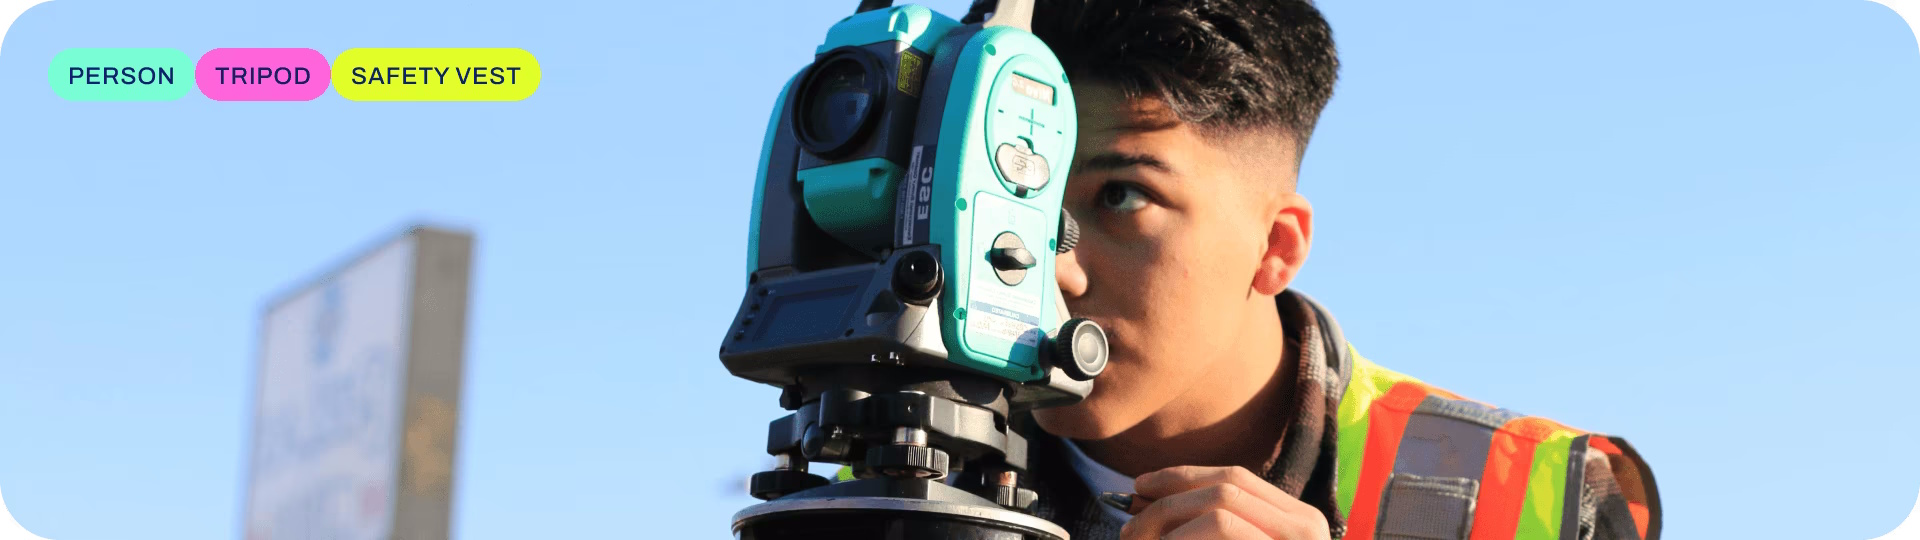
\includegraphics[width=\linewidth]{klassifizierung}
    \caption[Beispiel Klassifizierung]{Beispiel Klassifizierung (https://github.com/ultralytics/docs/releases/download/0/image-classification-examples.avif)}\label{beispiel_klassifizierung}
\end{figure}

\begin{figure}[H]
    \centering
    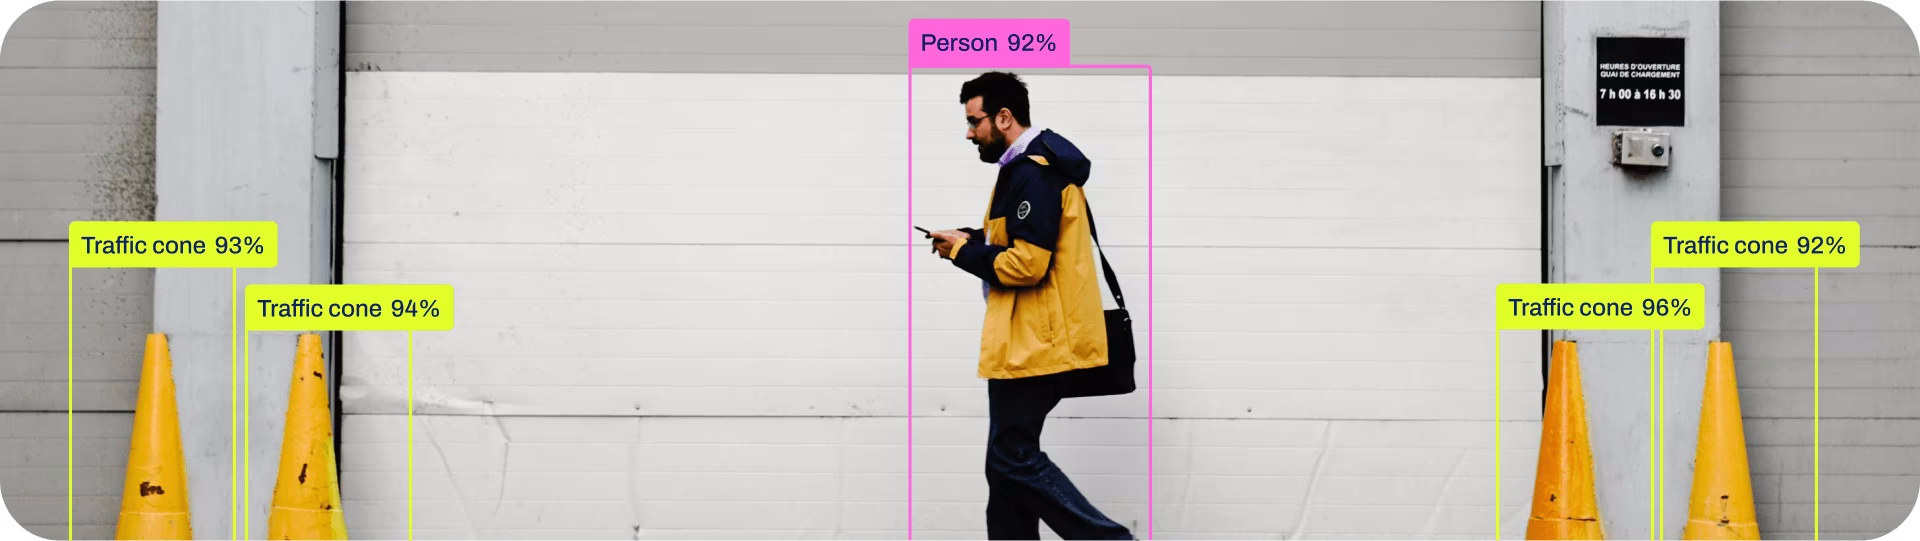
\includegraphics[width=\linewidth]{objekterkennung}
    \caption[Beispiel Objekterkennung]{Beispiel Objekterkennung (https://github.com/ultralytics/docs/releases/download/0/object-detection-examples.avif)}\label{beispiel_objekterkennung}
\end{figure}

\begin{figure}[H]
    \centering
    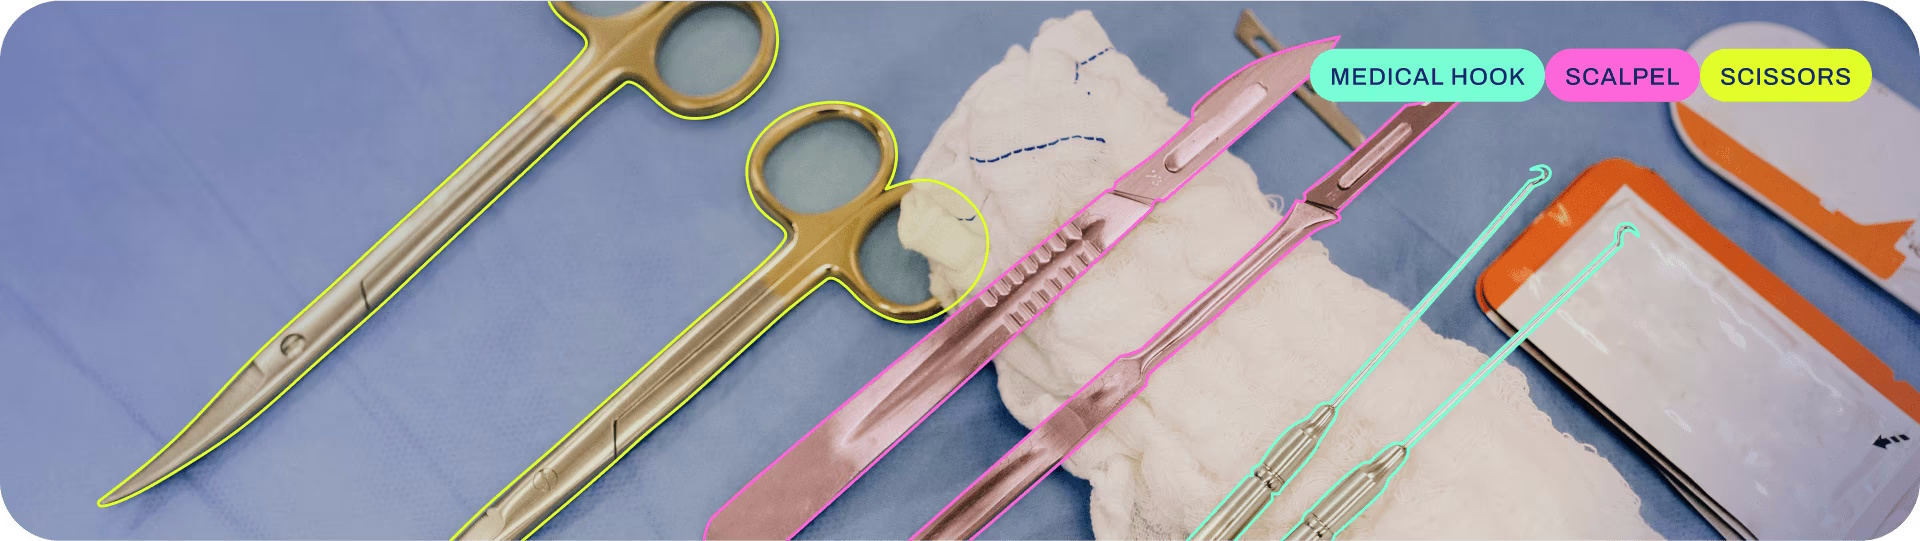
\includegraphics[width=\linewidth]{segmentierung}
    \caption[Beispiel Segmentierung]{Beispiel Segmentierung (https://github.com/ultralytics/docs/releases/download/0/instance-segmentation-examples.avif)}\label{beispiel_segmentierung}
\end{figure}

YOLO wurde seit seiner ersten Veröffentlichung kontinuierlich weiterentwickelt. 
Die frühen Versionen, wie YOLOv1 bis YOLOv3, legten den Grundstein für schnelle Erkennung. 
Ab YOLOv4 wurden weitere Optimierungen eingeführt, die vor allem das Training auf eigenen Datensätzen vereinfachten. 
Mit YOLOv5, das von der Firma Ultralytics gepflegt wird, wurde die Nutzung nochmals zugänglicher und die verschiedenen Modellgrößen wurden eingeführt.
Die Modellgrößen unterscheiden sich im Umfang der enthaltenen Parameter und bestimmen damit die Lauffähigkeit und Performance basierend auf den verfügbaren Hardwareressourcen.
Es gibt die Modellgrößen: \gq{n} (nano), \gq{s} (small), \gq{m} (medium), \gq{l} (large) und \gq{x} (extra large).
Neuere Versionen wie YOLOv6 bis YOLOv8 unterstützen neben der Objekterkennung auch Segmentierungs- und Tracking-Aufgaben.
\newPar
In diesem Projekt wurde sich für Version YOLOv11 in der Variante \gq{n} entschieden, also YOLOv11n.
Diese Modellvariante ist besonders kompakt und eignet sich dadurch gut für Anwendungen mit begrenzten Ressourcen.
Besonders ausschlaggebend für diese Entscheidung war die hohe Genauigkeit bei der Erkennung und Lokalisierung von Objekten (also bei der Berechnung der Bounding Boxes),
sowie die Performance auf ressourcenarmen Systemen, da das Training und die Inferenz zuerst innerhalb einer virtuellen Maschine durchgeführt wurde.
\newPar
Inferenz bezeichnet bei bildverarbeitenden Modellen den Prozess, bei dem ein trainiertes Modell neue, bisher unbekannte Bilddaten analysiert und daraus eine 
Vorhersage oder Entscheidung ableitet. Dabei greift das Modell auf das Wissen zurück, das es während des Trainings mit zahlreichen Beispielen (den Trainingsdaten) gelernt hat. 
Damit eine Inferenz durchgeführt werden kann, braucht es zunächst ein fertig trainiertes Modell sowie passende Eingabedaten, also ein neues Bild.
Zusätzlich ist eine geeignete Rechenumgebung notwendig. Oft wird dazu spezialisierte Hardware wie GPUs eingesetzt. da die Verarbeitung von Bilddaten rechenintensiv sein kann.
Mit passend ausgewählten und angepassten Modellen ist es jedoch auch möglich, Inferenz auf ressourcenärmeren Systeme auszuführen.
Inferenz ist damit der praktische Einsatz des zuvor gelernten Modells, etwa um Objekte zu erkennen, Bilder zu klassifizieren oder bestimmte Bildbereiche zu segmentieren.
\newPar
Die YOLO-Modelle sind bereits in der Lage, eine Vielzahl von vortrainierten Klassen zu erkennen, können aber für spezielle benutzerdefinierte Klassen nachtrainiert werden.
Genau dies ist ein Kernaspekt dieses Projektes und Basis der Entscheidung für YOLO als Modellframework.
\cite{yolo_docu}